\section{Windows -- SageCrypt}
\subsection{Introduction}
Sage est une nouvelle famille de ransomware, dérivée de CryLocker.\\
%TODO: topo ransomware

SHA-256 du sample :
\begin{lstlisting}
50624b1338349dcab4ad8345e0100ea75d3b643ef1e3a487b32fd711418b281b
\end{lstlisting}

\subsection{Les outils}
Les principaux outils utilisés pour réaliser cette analyse ont été
le logiciel de virtualisation \href{https://www.virtualbox.org/}{\textit{VirtualBox}},
le debugger \href{http://x64dbg.com}{\textit{x64dbg}},
l'utilitaire
\href{https://technet.microsoft.com/en-US/sysinternals/processmonitor.aspx}
{\textit{ProcessMonitor}},
l'éditeur hexadécimal \href{https://mh-nexus.de/en/hxd/}{\textit{HxD}},
le désassembleur \href{https://github.com/radare/radare2}{\textit{Radare2}}.\\

\subsection{Analyse}
\paragraph{Analyse basique}

\begin{lstlisting}
sage: PE32 executable (GUI) Intel 80386, for MS Windows
\end{lstlisting}
Exécutable au format PE (Portable Executable) 32-bit pour Windows.\\
\ \\
Côté \textit{strings}, rien d'intéressant :
\begin{lstlisting}
[...]
xcludeIe
MANDize
%04X%iArc
;*.baon-fiMAND
iarc.in
\Tran
ot s
clude
ange
efault)
%COMMANas receut w
IDPomes
ting
X%04Error
mmandd probl
ossiblips_rt
You auted coutpeck youges,on f
le typeuration
_ABO regi
std@@
Conf
ma.t
[...]
\end{lstlisting}
Aucune chaîne de caractères intelligible, ni aucune chaîne concernant une rançon
quelconque. On peut supposer que l'exécutable fait donc usage d'obfuscation au
moins pour les chaînes de caractères.\\

Pour avoir une meilleure idée de ce que peut faire le sample, dresser une liste
des fonctions qu'il importe (de KERNEL32.dll et NTDLL.dll en l'occurence,
bibliothèques incontournables pour les exécutables Windows).\\
Radare2 fait cela très bien :
\begin{lstlisting}
[0x0041d1e0]> ii | grep KERNEL32
ordinal=001 plt=0x0041e03c bind=NONE type=FUNC name=KERNEL32.dll_CloseHandle
ordinal=002 plt=0x0041e040 bind=NONE type=FUNC name=KERNEL32.dll_ResumeThread
ordinal=003 plt=0x0041e044 bind=NONE type=FUNC name=KERNEL32.dll_VirtualAlloc
ordinal=004 plt=0x0041e048 bind=NONE type=FUNC name=KERNEL32.dll_ReadProcessMemory
ordinal=005 plt=0x0041e04c bind=NONE type=FUNC name=KERNEL32.dll_SetConsoleMode
ordinal=006 plt=0x0041e050 bind=NONE type=FUNC name=KERNEL32.dll_SetProcessWorkingSetSize
ordinal=007 plt=0x0041e054 bind=NONE type=FUNC name=KERNEL32.dll_ReadFileEx
ordinal=008 plt=0x0041e058 bind=NONE type=FUNC name=KERNEL32.dll_GetModuleHandleA
ordinal=009 plt=0x0041e05c bind=NONE type=FUNC name=KERNEL32.dll_lstrcpynA
ordinal=010 plt=0x0041e060 bind=NONE type=FUNC name=KERNEL32.dll_GetProcAddress
ordinal=011 plt=0x0041e064 bind=NONE type=FUNC name=KERNEL32.dll_GetStartupInfoA
ordinal=012 plt=0x0041e068 bind=NONE type=FUNC name=KERNEL32.dll_SetEnvironmentVariableA
ordinal=013 plt=0x0041e06c bind=NONE type=FUNC name=KERNEL32.dll_Sleep
ordinal=014 plt=0x0041e070 bind=NONE type=FUNC name=KERNEL32.dll_SetStdHandle
ordinal=015 plt=0x0041e074 bind=NONE type=FUNC name=KERNEL32.dll_SetEvent
ordinal=016 plt=0x0041e078 bind=NONE type=FUNC name=KERNEL32.dll_ProcessIdToSessionId
ordinal=017 plt=0x0041e058 bind=NONE type=FUNC name=KERNEL32.dll_GetModuleHandleA
ordinal=018 plt=0x0041e080 bind=NONE type=FUNC name=KERNEL32.dll_LoadLibraryA

0x0041d1e0]> ii | grep NTDLL
ordinal=001 plt=0x0041e100 bind=NONE type=FUNC name=NTDLL.dll_isprint
ordinal=002 plt=0x0041e104 bind=NONE type=FUNC name=NTDLL.dll_iswdigit
ordinal=003 plt=0x0041e108 bind=NONE type=FUNC name=NTDLL.dll_RtlUnwind
ordinal=004 plt=0x0041e10c bind=NONE type=FUNC name=NTDLL.dll___toascii
ordinal=005 plt=0x0041e110 bind=NONE type=FUNC name=NTDLL.dll_strtol
ordinal=006 plt=0x0041e114 bind=NONE type=FUNC name=NTDLL.dll__CIsqrt
ordinal=007 plt=0x0041e118 bind=NONE type=FUNC name=NTDLL.dll_RtlMoveMemory
\end{lstlisting}
Première remarque, la liste est courte. Deuxième remarque, avec les fonctions
ici listées, difficile d'imaginer comment un ransomware pourrait mener à bien sa
mission (c'est-à-dire chiffrer des fichiers sans fonctions liées à la gestion
de fichiers).
Là encore, probable obfuscation. VirtuallAlloc et GetProcAddress sont
importées, ce qui permet tout à fait de charger du code (stocké compressé ou
chiffré) lors de l'exécution.

\paragraph{Obfuscation}
La première partie du main de Sage utilise une simple technique
pour rendre la lecture du code un peu plus pénible. Toutes les
4 à 10 instructions, un appel à une fonction s'occupant de modifier
la valeur du registre EIP, à la manière d'une instruction \textit{jmp}.
\begin{figure}[H]
  \center
  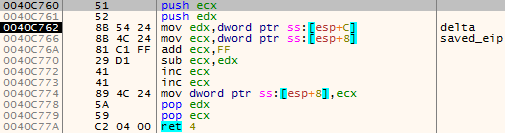
\includegraphics[width=350pt]{obf_func.png}
  \caption{Fonction utilisée pour exécuter une instruction \textit{jmp} de
    manière détournée.}
  \label{fig:func}
\end{figure}

\begin{figure}[H]
  \center
  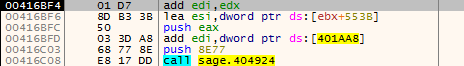
\includegraphics[width=350pt]{obf_usage.png}
  \caption{Utilisation de la fonction pour rendre le flot d'exécution plus
    difficile à suivre.}
  \label{fig:usage}
\end{figure}
\ \\
L'essentiel du code du ransomware est stocké chiffré en mémoire.\\
Le chargement du code se fait en 2 parties. D'abord un \textit{stub}
est déchiffré (combinaisons de xor/add) puis exécuté. Ce stub se charge
ensuite de déchiffrer (à l'aide de RC4) la troisième partie, qui
est la partie principale puis de passer l'exécution à cette partie.\\
\ \\
processus / executable -> deplacement dans roaming\\

\paragraph{Main}
\subparagraph{Locale check}
Lors des attaques cybers, il y a des pays moins concernés que d'autres.
Sage vérifie donc d'après le layout du clavier utilisé sur la machine, dans
quel pays se situe la machine sur laquelle il est en train de s'exécuter.
Si ce layout correspond à un des suivants, alors il s'arrête avant de chiffrer
quoi que ce soit :
\begin{itemize}
\item Biélorusse
\item Kazakh
\item Russe
\item Ukrainien
\item Ouzbek
\item Sakha
\end{itemize}

\subparagraph{Location fingerprinting}
maps.googleapis.com, SSID et MAC pour la localisation

\subparagraph{Persistance}
En ce qui concerne la persistance (l'exécution de lui-même au démarrage),
Sage fait usage des tâches planifiées de Windows. Après s'être copié dans
le dossier \textbf{AppData\textbackslash Roaming\textbackslash}, Sage ajoute une tâche dans la liste
de manière à relancer l'exécution de son binaire à chaque nouvelle connexion
d'un utilisateur sur la machine. Ceci permet de s'assurer que la machine
reste inutilisable après l'infection et ce jusqu'à ce que la rançon
soit payée.\\

\begin{figure}[H]
  \center
  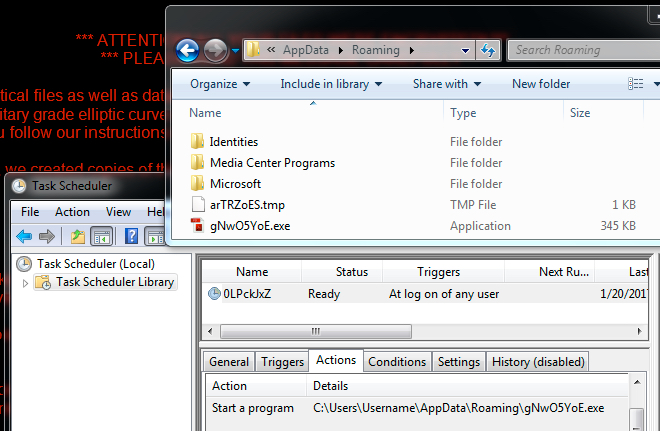
\includegraphics[width=350pt]{persis_task.jpg}
  \caption{Binaire de sage et tâche planifiée utilisée pour maintenir
    l'exécution au démarrage.}
  \label{fig:task}
\end{figure}


\subparagraph{Debug \& Canary file}
Un des restes de plusieurs fonctionnalités de debug
\begin{lstlisting}
if (CreateFileW(L"", 0x80000000, 1u, 0, 3u, 0, 0) == INVALID_HANDLE_VALUE)
{
	// Chiffrement des fichiers
}
\end{lstlisting}

\paragraph{Extension whitelist}
Pour éviter de rendre le système d'exploitation inutilisable en chiffrant des
fichiers critiques, les ransomwares se contentent de chiffrer uniquement les
fichiers dont les noms contiennent les extensions les plus couramment utilisées.\\
En ce qui concerne Sage, cette liste est la suivante :
\begin{lstlisting}
.dat .mx0 .cd .pdb .xqx .old .cnt .rtp .qss .qst .fx0 .fx1 .ipg .ert .pic .img
.cur .fxr .slk .m4u .mpe .mov .wmv .mpg .vob .mpeg .3g2 .m4v .avi .mp4 .flv
.mkv .3gp .asf .m3u .m3u8 .wav .mp3 .m4a .m .rm .flac .mp2 .mpa .aac .wma .djv
.pdf .djvu .jpeg .jpg .bmp .png .jp2 .lz .rz .zipx .gz .bz2 .s7z .tar .7z .tgz
.rar .zip .arc .paq .bak .set .back .std .vmx .vmdk .vdi .qcow .ini .accd .db
.sqli .sdf .mdf .myd .frm .odb .myi .dbf .indb .mdb .ibd .sql .cgn .dcr .fpx
.pcx .rif .tga .wpg .wi .wmf .tif .xcf .tiff .xpm .nef .orf .ra .bay .pcd .dng
.ptx .r3d .raf .rw2 .rwl .kdc .yuv .sr2 .srf .dip .x3f .mef .raw .log .odg .uop
.potx .potm .pptx .rss .pptm .aaf .xla .sxd .pot .eps .as3 .pns .wpd .wps .msg
.pps .xlam .xll .ost .sti .sxi .otp .odp .wks .vcf .xltx .xltm .xlsx .xlsm
.xlsb .cntk .xlw .xlt .xlm .xlc .dif .sxc .vsd .ots .prn .ods .hwp .dotm .dotx
.docm .docx .dot .cal .shw .sldm .txt .csv .mac .met .wk3 .wk4 .uot .rtf .sldx
.xls .ppt .stw .sxw .dtd .eml .ott .odt .doc .odm .ppsm .xlr .odc .xlk .ppsx
.obi .ppam .text .docb .wb2 .mda .wk1 .sxm .otg .oab .cmd .bat .h .asx .lua .pl
.as .hpp .clas .js .fla .py .rb .jsp .cs .c .jar .java .asp .vb .vbs .asm .pas
.cpp .xml .php .plb .asc .lay6 .pp4 .pp5 .ppf .pat .sct .ms11 .lay .iff .ldf
.tbk .swf .brd .css .dxf .dds .efx .sch .dch .ses .mml .fon .gif .psd .html
.ico .ipe .dwg .jng .cdr .aep .aepx .123 .prel .prpr .aet .fim .pfb .ppj .indd
.mhtm .cmx .cpt .csl .indl .dsf .ds4 .drw .indt .pdd .per .lcd .pct .prf .pst
.inx .plt .idml .pmd .psp .ttf .3dm .ai .3ds .ps .cpx .str .cgm .clk .cdx .xhtm
.cdt .fmv .aes .gem .max .svg .mid .iif .nd .2017 .tt20 .qsm .2015 .2014 .2013
.aif .qbw .qbb .qbm .ptb .qbi .qbr .2012 .des .v30 .qbo .stc .lgb .qwc .qbp
.qba .tlg .qbx .qby .1pa .ach .qpd .gdb .tax .qif .t14 .qdf .ofx .qfx .t13 .ebc
.ebq .2016 .tax2 .mye .myox .ets .tt14 .epb .500 .txf .t15 .t11 .gpc .qtx .itf
.tt13 .t10 .qsd .iban .ofc .bc9 .mny .13t .qxf .amj .m14 ._vc .tbp .qbk .aci
.npc .qbmb .sba .cfp .nv2 .tfx .n43 .let .tt12 .210 .dac .slp .qb20 .saj .zdb
.tt15 .ssg .t09 .epa .qch .pd6 .rdy .sic .ta1 .lmr .pr5 .op .sdy .brw .vnd .esv
.kd3 .vmb .qph .t08 .qel .m12 .pvc .q43 .etq .u12 .hsr .ati .t00 .mmw .bd2 .ac2
.qpb .tt11 .zix .ec8 .nv .lid .qmtf .hif .lld .quic .mbsb .nl2 .qml .wac .cf8
.vbpf .m10 .qix .t04 .qpg .quo .ptdb .gto .pr0 .vdf .q01 .fcr .gnc .ldc .t05
.t06 .tom .tt10 .qb1 .t01 .rpf .t02 .tax1 .1pe .skg .pls .t03 .xaa .dgc .mnp
.qdt .mn8 .ptk .t07 .chg .#vc .qfi .acc .m11 .kb7 .q09 .esk .09i .cpw .sbf .mql
.dxi .kmo .md .u11 .oet .ta8 .efs .h12 .mne .ebd .fef .qpi .mn5 .exp .m16 .09t
.00c .qmt .cfdi .u10 .s12 .qme .int? .cf9 .ta5 .u08 .mmb .qnx .q07 .tb2 .say
.ab4 .pma .defx .tkr .q06 .tpl .ta2 .qob .m15 .fca .eqb .q00 .mn4 .lhr .t99
.mn9 .qem .scd .mwi .mrq .q98 .i2b .mn6 .q08 .kmy .bk2 .stm .mn1 .bc8 .pfd .bgt
.hts .tax0 .cb .resx .mn7 .08i .mn3 .ch .meta .07i .rcs .dtl .ta9 .mem .seam
.btif .11t .efsl .$ac .emp .imp .fxw .sbc .bpw .mlb .10t .fa1 .saf .trm .fa2
.pr2 .xeq .sbd .fcpa .ta6 .tdr .acm .lin .dsb .vyp .emd .pr1 .mn2 .bpf .mws
.h11 .pr3 .gsb .mlc .nni .cus .ldr .ta4 .inv .omf .reb .qdfx .pg .coa .rec .rda
.ffd .ml2 .ddd .ess .qbmd .afm .d07 .vyr .acr .dtau .ml9 .bd3 .pcif .cat .h10
.ent .fyc .p08 .jsd .zka .hbk .mone .pr4 .qw5 .cdf .gfi .cht .por .qbz .ens
.3pe .pxa .intu .trn .3me .07g .jsda .2011 .fcpr .qwmo .t12 .pfx .p7b .der .nap
.p12 .p7c .crt .csr .pem .gpg .key
\end{lstlisting}

\paragraph{Chiffrement}
Sage se démarque des autres ransomwares en ce qui concerne le chiffrement
puisqu'il fait usage de la cryptographie sur les courbes elliptiques ainsi que
de l'algorithme ChaCha pour chiffrer les fichiers de l'utilisateur, ce qui
n'est pas commun.\\
ChaCha est un algortihme de chiffrement à flot dérivé de Salsa20; Sage l'utilise
pour chiffrer le contenu des fichiers.\\
Chaque fichier cible est renommé et chiffré avec une clé ChaCha
choisie aléatoirement, et cette clé est ensuite stockée à la fin du fichier
chiffré. Cette clé n'est évidemment pas stockée tel quel dans le fichier, ce
sont en fait deux parties qui permettent, si on possède une valeur secrète, de
retrouver la clé utilisée pour chiffrer le fichier, qui sont stockées.\\
\ \\
Les calculs sont faits sur la courbe elliptique \textit{Curve25519} (d'équation
$y^2 = x^3 + 486662*x^2 + x$, sur $F_p = GF(2^{255} - 19)$), qui est
une courbe populaire pour plusieurs raisons (sécurité, rapidité des calculs,
propriétés liées à la génération d'éléments aléatoires) et qui est conçue pour
être utilisée par le protocole ECDH (Elliptic Curve Diffie-Hellman).\\
Dans la suite, on notera $F_p = GF(2^{255} - 19)$ et $G$ le point de la courbe
$Curve25519$ admettant $x = 9$. Enfin, le ransomware a connaissance de
$Q_s = k_s * G$, la partie publique de l'extorqueur utilisée lors de la création
du secret partagé.\\
Le chiffrement d'un fichier se déroule comme ceci :
\begin{itemize}
\item On génère $k_c \in F_p$ aléatoirement
\item On calcule le point $Q_c = k_c * G$
\item On calcule le secret partagé $S = k_c * Q_s = (k_c * k_s) * G$
\item On dérive du secret partagé, un entier $sh \in F_p$
\item On calcule le point $P = sh * G$
\item On génère $n \in F_p$ aléatoirement
\item On calcule les points $chacha\_key = n * P = (n * sh) * G$ et $chacha\_pub = n * G$
\item On chiffre le fichier en utilisant ChaCha avec la clé $chacha\_key$ (note interpretation)
\item On ajoute les valeurs de $Q_c$ et $chacha\_pub$ à la fin du fichier
\end{itemize}
\ \\

Ce qui produit, en pratique, un fichier de la forme :
\begin{figure}[H]
  \center
  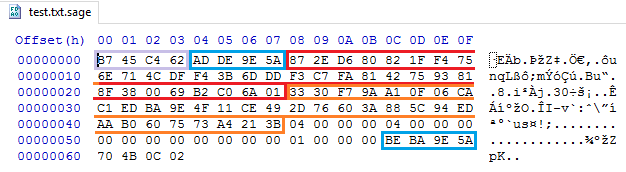
\includegraphics[width=350pt]{dump_file.png}
  \caption{Contenu d'un fichier après avoir été chiffré par Sage.}
  \label{fig:file}
\end{figure}
\ \\
Légende :
\begin{itemize}
\item Mauve : Contenu chiffré du fichier original
\item Rouge : $Q_c$
\item Orange : $chacha\_pub$
\item Bleu : Valeurs constantes
\end{itemize}

Petite note sur le déchiffrement; il est nécéssaire de connaître la valeur
de $k_s$ pour pouvoir déchiffrer les fichiers. Cette valeur n'est stockée
nulle part dans le binaire et on peut donc supposer que seul l'auteur du
ransomware la possède, évidemment.\\
Le déchiffrement d'un fichier se déroule comme ceci :
\begin{itemize}
\item On récupère les valeurs $Q_c$ et $chacha\_pub$
\item On calcule le secret partagé $S = k_s * Q_c = (k_s * k_c) * G$
\item On dérive du secret partagé, l'entier $sh \in F_p$
\item On calcule $chacha\_key = sh * chacha\_pub = (sh * n) * G$
\item On déchiffre le fichier en utilisant ChaCha avec la clé $chacha\_key$
\end{itemize}
